% 2.1-2.5 Study Guide -- August 2026
%
% PRIVATE MAP (comments never appear in the PDF; delete this block if you ever
% hand out the .tex source itself).  Guide number = textbook problem:
%   1=2.1#1   2=2.1#5   3=2.1#9   4=2.1#12  5=2.1#13  6=2.1#14  7=2.1#16
%   8=2.1#17  9=2.1#21  10=2.1#25 11=2.1#33 12=2.1#35 13=2.1#37
%   14=2.3#13 15=2.3#45 16=2.3#49 17=2.3#62
%   18=2.4#7  19=2.4#9  20=2.4#21 21=2.4#23 22=2.4#39
%   23=2.5#1  24=2.5#3  25=2.5#7  26=2.5#8  27=2.5#10
%   28=2.5#20 29=2.5#23 30=2.5#27 31=2.5#33 32=2.5#55
%
% WORK SPACE: change the four lengths in \wsS \wsM \wsL \wsG below to make every
% blank on the worksheet bigger or smaller at once.
%
\documentclass[11pt]{article}
\usepackage[margin=1in]{geometry}
\usepackage{amsmath,amssymb}
\usepackage{enumitem}
\usepackage{tikz}

% ---- blank space for students to work in ----
\newcommand{\wsS}{\vspace*{3cm}}    % one- or two-step problem
\newcommand{\wsM}{\vspace*{4.5cm}}  % several steps, or parts (a)(b)(c)
\newcommand{\wsL}{\vspace*{6.5cm}}  % sketch a graph / long argument
\newcommand{\wsG}{\vspace*{2cm}}    % short answers beside a printed graph

\colorlet{curve}{blue!55!black}
\tikzset{
  hole/.style={circle,draw=curve,fill=white,inner sep=1.5pt,line width=.7pt},
  fdot/.style={circle,fill=curve,inner sep=1.8pt},
  cline/.style={draw=curve,line width=1pt}
}
% axes: {xmin}{xmax}{ymin}{ymax}
\newcommand{\gaxes}[4]{%
  \draw[->,gray] (#1,0) -- (#2,0) node[below,black,font=\scriptsize] {$x$};
  \draw[->,gray] (0,#3) -- (0,#4) node[right,black,font=\scriptsize] {$y$};
  \foreach \tx in {#1,...,#2} {\draw[gray] (\tx,-0.12) -- (\tx,0.12);}
  \foreach \ty in {#3,...,#4} {\draw[gray] (-0.12,\ty) -- (0.12,\ty);}
}

% ---- reusable figures (11 and 24 share a graph; 13 and 25 share a graph) ----
\newcommand{\figJump}{
\begin{tikzpicture}[scale=0.58]
  \gaxes{-4}{7}{-2}{5}
  \draw[cline] plot[smooth] coordinates {(-3.5,0.5)(-3,0.55)(-2,0.8)(-1,1.3)(0,2.1)(1,2.75)(1.5,2.9)(2,2.98)};
  \draw[cline] plot[smooth] coordinates {(2,1)(2.5,1.1)(3,1.45)(3.5,1.95)(4,2.3)(4.5,2.45)(5,2.5)(5.5,2.45)};
  \node[hole] at (2,3) {}; \node[hole] at (2,1) {};
\end{tikzpicture}}

\newcommand{\figVee}{
\begin{tikzpicture}[scale=0.58]
  \gaxes{-4}{5}{-2}{7}
  \draw[cline] plot[smooth] coordinates {(-3,4.6)(-2,4.1)(-1,3.6)(0,3)(0.5,2.55)(1,2.05)(1.5,1.55)(2,1)};
  \draw[cline] plot[smooth] coordinates {(2,1)(2.3,1.7)(2.6,2.15)(3,2.5)(3.5,2.8)(4,3)};
  \node[hole] at (2,1) {}; \node[fdot] at (2,4) {};
\end{tikzpicture}}

\newcommand{\figSaw}{
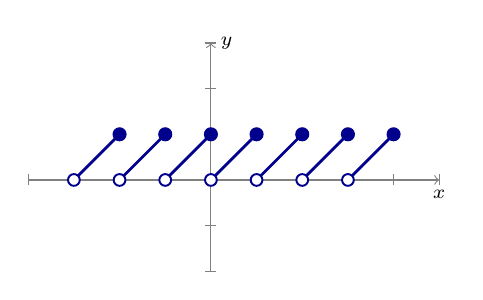
\begin{tikzpicture}[scale=0.58]
  \gaxes{-4}{5}{-2}{3}
  \foreach \n in {-3,-2,-1,0,1,2,3} {
    \draw[cline] (\n,0) -- ({\n+1},1);
    \node[hole] at (\n,0) {};
    \node[fdot] at ({\n+1},1) {};
  }
\end{tikzpicture}}

\newcommand{\figInf}{
\begin{tikzpicture}[scale=0.58]
  \gaxes{-3}{7}{-6}{7}
  \draw[dashed,gray!80] (2,-6.3) -- (2,6.8);
  \draw[cline] plot[smooth] coordinates {(0,0)(0.3,-0.25)(0.7,-0.7)(1,-1.2)(1.3,-2)(1.5,-3)(1.62,-4.2)(1.7,-5.5)(1.75,-6.3)};
  \draw[cline] plot[smooth] coordinates {(2.25,6.3)(2.35,5)(2.5,3.6)(2.7,2.4)(3,1.7)(3.5,1.15)(4,0.9)(5,0.65)(6,0.5)(6.5,0.45)};
  \node[hole] at (0,0) {};
\end{tikzpicture}}

\newcommand{\figBoth}{
\begin{tikzpicture}[scale=0.58]
  \gaxes{-4}{7}{-3}{7}
  \draw[dashed,gray!80] (2,-3) -- (2,6.8);
  \draw[cline] plot[smooth] coordinates {(-3,-0.7)(-2,-0.6)(-1,-0.45)(-0.25,0)(0.3,0.5)(0.8,1.2)(1.2,2.2)(1.5,3.5)(1.7,5)(1.8,6.5)};
  \draw[cline] plot[smooth] coordinates {(2.2,6.5)(2.35,5)(2.6,3.2)(2.9,2)(3.2,1)(3.6,0)(4.2,-0.7)(5,-1.05)(5.8,-1.2)};
\end{tikzpicture}}

\newcommand{\figHole}{
\begin{tikzpicture}[scale=0.58]
  \gaxes{-4}{4}{-2}{4}
  \draw[cline] plot[smooth] coordinates {(-3,1.8)(-2,1.65)(-1,1.4)(0,1)(0.5,0.8)(1,0.6)(1.5,0.35)(1.8,0.18)(2,0)};
  \node[hole] at (0,1) {}; \node[hole] at (2,0) {};
\end{tikzpicture}}

\newlist{probs}{itemize}{1}
\setlist[probs]{leftmargin=2.6em,itemsep=6pt,topsep=4pt,label={}}
\newcommand{\prob}[1]{\item[\textbf{#1.}]}
\newcommand{\headnote}[1]{\smallskip\noindent\textit{#1}\par\nopagebreak}

\title{\textbf{2.1--2.5 Study Guide}}
\author{}
\date{August 2026}

\begin{document}
\maketitle
\vspace{-2.5em}
\begin{center}\small Recommended Continued Practice (not for credit)\end{center}
\vspace{1em}

\headnote{Find the limit.}
\begin{probs}
  \prob{1} $\displaystyle\lim_{x\to-2}(3x-1)$ \wsS
  \prob{2} $\displaystyle\lim_{x\to100}7$ \wsS
  \prob{3} $\displaystyle\lim_{x\to-1}\frac{x+4}{2x+1}$ \wsS
\end{probs}

\headnote{Use an algebraic simplification to help find the limit, if it exists.}
\begin{probs}
  \prob{4} $\displaystyle\lim_{x\to-1}\frac{(x+1)(x^{2}+3)}{x+1}$ \wsS
  \prob{5} $\displaystyle\lim_{x\to2}\frac{x^{2}-4}{x-2}$ \wsS
  \prob{6} $\displaystyle\lim_{x\to3}\frac{2x^{3}-6x^{2}+x-3}{x-3}$ \wsM
  \prob{7} $\displaystyle\lim_{r\to-3}\frac{r^{2}+2r-3}{r^{2}+7r+12}$ \wsM
  \prob{8} $\displaystyle\lim_{k\to4}\frac{k^{2}-16}{\sqrt{k}-2}$ \wsM
  \prob{9} $\displaystyle\lim_{h\to-2}\frac{h^{3}+8}{h+2}$ \wsM
\end{probs}

\headnote{Find each limit, if it exists:
\quad (a) $\displaystyle\lim_{x\to a^{-}}f(x)$ \quad (b) $\displaystyle\lim_{x\to a^{+}}f(x)$ \quad (c) $\displaystyle\lim_{x\to a}f(x)$}
\begin{probs}
  \prob{10} $f(x)=\dfrac{|x-4|}{x-4};\qquad a=4$ \wsM
\end{probs}

\headnote{Refer to the graph to find each limit, if it exists:
\quad (a) $\displaystyle\lim_{x\to2^{-}}f(x)$ \quad (b) $\displaystyle\lim_{x\to2^{+}}f(x)$ \quad (c) $\displaystyle\lim_{x\to2}f(x)$
\quad (d) $\displaystyle\lim_{x\to0^{-}}f(x)$ \quad (e) $\displaystyle\lim_{x\to0^{+}}f(x)$ \quad (f) $\displaystyle\lim_{x\to0}f(x)$}
\begin{probs}
  \prob{11} \raisebox{-0.5\height}{\figVee} \wsG
  \prob{12} \raisebox{-0.5\height}{\figSaw} \wsG
  \prob{13} \raisebox{-0.5\height}{\figInf} \wsG
\end{probs}

\headnote{Use theorems on limits to find the limit, if it exists.}
\begin{probs}
  \prob{14} $\displaystyle\lim_{x\to-2}\bigl(3x^{3}-2x+7\bigr)$ \wsS
  \prob{15} $\displaystyle\lim_{x\to3^{+}}\frac{\sqrt{(x-3)^{2}}}{x-3}$ \wsM
\end{probs}

\headnote{Find each limit, if it exists:
\quad (a) $\displaystyle\lim_{x\to a^{-}}f(x)$ \quad (b) $\displaystyle\lim_{x\to a^{+}}f(x)$ \quad (c) $\displaystyle\lim_{x\to a}f(x)$}
\begin{probs}
  \prob{16} $f(x)=\sqrt{5-x};\qquad a=5$ \wsM
\end{probs}

\headnote{Use the sandwich theorem to verify the limit.}
\begin{probs}
  \prob{17} $\displaystyle\lim_{x\to0}\frac{|x|}{\sqrt{x^{4}+4x^{2}+7}}=0$
  \quad \textit{(Hint: Use $f(x)=0$ and $g(x)=|x|$.)} \wsM
\end{probs}

\headnote{For the given $f(x)$, express each of the following limits as $\infty$, $-\infty$, or DNE (Does Not Exist):
\quad (a) $\displaystyle\lim_{x\to a^{-}}f(x)$ \quad (b) $\displaystyle\lim_{x\to a^{+}}f(x)$ \quad (c) $\displaystyle\lim_{x\to a}f(x)$}
\begin{probs}
  \prob{18} $f(x)=\dfrac{2x^{2}}{x^{2}-x-2};\qquad a=-1$ \wsM
  \prob{19} $f(x)=\dfrac{1}{x(x-3)^{2}};\qquad a=3$ \wsM
\end{probs}

\headnote{Find the limit, if it exists.}
\begin{probs}
  \prob{20} $\displaystyle\lim_{x\to\infty}\sqrt[3]{\frac{8+x^{2}}{x(x+1)}}$ \wsM
  \prob{21} $\displaystyle\lim_{x\to\infty}\sin x$ \wsS
\end{probs}

\headnote{A function $f$ satisfies the given conditions. Sketch a possible graph for $f$, assuming that it does not cross a horizontal asymptote.}
\begin{probs}
  \prob{22}
  $\displaystyle\lim_{x\to-\infty}f(x)=-2;\qquad \lim_{x\to\infty}f(x)=-2;$\\[2pt]
  $\displaystyle\lim_{x\to3^{-}}f(x)=\infty;\qquad\ \ \lim_{x\to3^{+}}f(x)=-\infty;$\\[2pt]
  $\displaystyle\lim_{x\to-1^{-}}f(x)=-\infty;\qquad \lim_{x\to-1^{+}}f(x)=\infty$ \wsL
\end{probs}

\headnote{The graph of a function $f$ is given. Classify the discontinuities of $f$ as removable, jump, or infinite.}
\begin{probs}
  \prob{23} \raisebox{-0.5\height}{\figJump} \wsG
  \prob{24} \raisebox{-0.5\height}{\figVee} \wsG
  \prob{25} \raisebox{-0.5\height}{\figInf} \wsG
  \prob{26} \raisebox{-0.5\height}{\figBoth} \wsG
  \prob{27} \raisebox{-0.5\height}{\figHole} \wsG
\end{probs}

\headnote{Show that $f$ is continuous at $a$.}
\begin{probs}
  \prob{28} $f(x)=\sqrt[3]{x^{2}+2};\qquad a=-5$ \wsM
\end{probs}

\headnote{Explain why $f$ is not continuous at $a$.}
\begin{probs}
  \prob{29} $f(x)=\dfrac{3}{x+2};\qquad a=-2$ \wsS
  \prob{30} $f(x)=\begin{cases}1 & \text{if } x\neq3\\ 0 & \text{if } x=3\end{cases}\qquad a=3$ \wsS
\end{probs}

\headnote{Find all numbers at which $f$ is discontinuous.}
\begin{probs}
  \prob{31} $f(x)=\dfrac{x-1}{x^{2}+x-2}$ \wsM
\end{probs}

\headnote{Verify the intermediate value theorem for $f$ on the stated interval $[a,b]$ by showing
that if $f(a)\le w\le f(b)$, then $f(c)=w$ for some $c$ in $[a,b]$.}
\begin{probs}
  \prob{32} $f(x)=x^{3}+1;\qquad [-1,2]$ \wsL
\end{probs}

%======================================================================
\section*{Tommy's Questions}
\noindent\textit{These two are written by us. Each one pulls several ideas together at once,
so show all of your work.}
\medskip

\noindent\textbf{Tommy 1.}\quad Every part of this problem happens at $x=3$.
\begin{enumerate}[label=\textbf{(\alph*)},leftmargin=2.8em,itemsep=6pt,topsep=5pt]
  \item $\displaystyle\lim_{x\to3}\frac{x^{2}-x-6}{x^{2}-9}$ \wsM
  \item $\displaystyle\lim_{h\to0}\frac{\sqrt{9+h}-3}{h}$ \wsM
  \item For $f(x)=\dfrac{2x-6}{|x-3|}$, find
        \ (i) $\displaystyle\lim_{x\to3^{-}}f(x)$,
        \ (ii) $\displaystyle\lim_{x\to3^{+}}f(x)$,
        \ (iii) $\displaystyle\lim_{x\to3}f(x)$. \wsL
  \item Use the sandwich theorem to find
        $\displaystyle\lim_{x\to3}\,(x-3)^{2}\sin\!\left(\frac{1}{x-3}\right)$. \wsM
\end{enumerate}

\bigskip
\noindent\textbf{Tommy 2.}\quad Let
$\displaystyle f(x)=\frac{x^{2}-4}{x^{2}-x-6}$.
\begin{enumerate}[label=\textbf{(\alph*)},leftmargin=2.8em,itemsep=6pt,topsep=5pt]
  \item Find every number at which $f$ is discontinuous, and classify each discontinuity
        as removable, jump, or infinite. \wsM
  \item Find $\displaystyle\lim_{x\to3^{-}}f(x)$ and $\displaystyle\lim_{x\to3^{+}}f(x)$. \wsM
  \item Find $\displaystyle\lim_{x\to\infty}f(x)$ and $\displaystyle\lim_{x\to-\infty}f(x)$,
        then state every vertical and horizontal asymptote of the graph of $f$.
        \textit{(Careful: not every discontinuity is a vertical asymptote.)} \wsM
  \item $f$ is continuous on $[0,2]$. Use the intermediate value theorem to show that
        $f(c)=\tfrac{1}{2}$ for some $c$ in $[0,2]$, and then find that $c$ exactly. \wsL
\end{enumerate}

\end{document}
